\documentclass[11pt,letterpaper]{article}

\usepackage[margin=1.15in]{geometry}
\usepackage[T1]{fontenc}
\usepackage[utf8]{inputenc}
\usepackage{lmodern}
\usepackage{amsmath,amssymb,amsthm}
\usepackage{booktabs}
\usepackage{graphicx}
\usepackage{array}
\usepackage{xcolor}
\usepackage{microtype}
\usepackage{listings}
\usepackage{caption}
\usepackage{enumitem}
\usepackage[hidelinks,breaklinks]{hyperref}
\usepackage{cleveref}

\definecolor{codebg}{gray}{0.96}
\definecolor{rulegray}{gray}{0.55}

\lstset{
  basicstyle=\ttfamily\footnotesize,
  backgroundcolor=\color{codebg},
  breaklines=true,
  columns=fullflexible,
  frame=leftline,
  framerule=1pt,
  rulecolor=\color{rulegray},
  xleftmargin=1em,
  framexleftmargin=1em,
  showstringspaces=false,
  keepspaces=true,
}

\theoremstyle{definition}
\newtheorem{definition}{Definition}
\newtheorem{invariant}{Invariant}[section]
\theoremstyle{plain}
\newtheorem{hypothesis}{Hypothesis}
\theoremstyle{remark}
\newtheorem{observation}{Observation}
\crefname{invariant}{Invariant}{Invariants}
\Crefname{invariant}{Invariant}{Invariants}
\crefname{definition}{Definition}{Definitions}
\Crefname{definition}{Definition}{Definitions}
\crefname{hypothesis}{Hypothesis}{Hypotheses}
\Crefname{hypothesis}{Hypothesis}{Hypotheses}
\crefname{observation}{Observation}{Observations}
\Crefname{observation}{Observation}{Observations}

\newcommand{\Dset}{\mathcal{D}}
\newcommand{\Aset}{\mathcal{A}}
\newcommand{\Sset}{\mathcal{S}}
\newcommand{\Tset}{\mathcal{T}}
\newcommand{\Kset}{\mathcal{K}}
\newcommand{\dbn}[1]{\textsc{db-#1}}
\newcommand{\code}[1]{\texttt{#1}}
\newcommand{\PASS}{\textsc{hold}}
\newcommand{\FAIL}{\textbf{\textsc{fail}}}

\title{\textbf{Conventions Live in the Harness}\\[0.35em]
\large Formalizing and Auditing a Text-to-SQL Reinforcement-Learning\\
Environment Suite Built Without a Reference Benchmark}
\author{}
\date{August 2026}

\begin{document}
\maketitle

\begin{abstract}
\noindent
We present \textbf{MIRROR-SQL}, a suite of thirteen relational database environments
($176$ tables, $19.4$\,GB of instance data) paired with $390$ human-authored
natural-language/SQL task instances, and use it to make an argument about how benchmark
quality is transmitted.

MIRROR-SQL was constructed in seventeen days with no reference corpus, no acceptance rubric, and
requirements that arrived during the build. We formalize each environment as a partially
observable Markov decision process $\langle \Sset, \Aset, \Omega, T, O, R, \gamma\rangle$ in
which partial observability is structural: the agent observes the schema and the utterance
but never the instance, so the optimal policy must reason about data it can reach only by
spending actions. We then state eight environment invariants as decidable predicates over the
artifact and check them with a released tool. Three hold; five fail. The corpus advertises $390$
gold actions and supplies $222$ distinct ones ($56.9\%$) at a $0.99$ normalized-similarity
threshold; its \code{complexity} field is constant across all $390$ instances; and all $390$
\code{expected\_output} values are prose rather than result relations, so no execution reward
is computable without re-execution.

The failures are not a random sample of possible defects. Each corresponds to a property that
Spider and BIRD supply implicitly \emph{through their evaluation harnesses} rather than
explicitly in any specification: executed ground truth, a difficulty scale, action
distinctness, and schema closure. We formulate this as the \emph{missing-convention
hypothesis}---an artifact built without a harness will lack the harness-borne conventions in
a predictable pattern---and argue that its practical corollary is to build the scoring
harness first, however trivial, because the harness is the mechanism that makes tacit
conventions explicit. Given that $52.8\%$ of BIRD Mini-Dev has been shown to contain
annotation errors~\cite{jin2026broken}, we further argue that a published invariant audit
should accompany any environment intended to supply reward signal.
\end{abstract}

\section{Introduction}
\label{sec:intro}

Text-to-SQL is a standard proving ground for tool-using language agents, and reinforcement
learning against execution feedback is now the dominant method for improving
them~\cite{pourreza2025reasoningsql,zhang2025rewardsql,graphrewardsql2025}. Such methods
require an \emph{environment}: a state space the agent can act on, a transition rule, and a
reward computable at training time. Most published text-to-SQL resources are datasets from
which an environment can be built. The distance between the two is short but consequential,
and it is where defects hide.

A dataset is judged by whether its examples are correct. An environment is judged by whether
its reward is computable, its action space is well-formed, and its state transitions are
defined. These are different properties, and a resource can satisfy the first while failing
the second in ways that no example-level inspection reveals.

This paper does three things. It formalizes a thirteen-environment text-to-SQL suite as a
POMDP, mapping every field of the delivered artifact onto a tuple element and identifying
which fields can and cannot serve as reward. It states eight environment invariants as
decidable predicates and reports the result of checking them. And it uses the pattern of
failures to argue a general point about how benchmark conventions propagate.

\paragraph{Contributions.}
\begin{enumerate}[leftmargin=1.5em,itemsep=2pt,topsep=3pt]
  \item A POMDP formalization (\Cref{sec:pomdp}) in which the schema/instance split
        \emph{is} the observation function, with an explicit field-to-element mapping.
  \item Eight environment invariants (\Cref{sec:invariants}) stated as first-order predicates
        over a shipped artifact, with a released checker.
  \item A measured audit (\Cref{sec:results}): five of eight invariants fail, each quantified,
        with the consequences for RL training derived.
  \item The missing-convention hypothesis (\Cref{sec:hypothesis}), which explains the pattern
        of failures and yields a construction rule.
  \item A remediation specification (\Cref{sec:remediation}) that repairs the environment
        without regenerating its instance data.
\end{enumerate}

\section{Related Work}
\label{sec:related}

\paragraph{Cross-domain text-to-SQL corpora.}
Spider~\cite{yu2018spider} established the cross-domain protocol---disjoint train and test
database sets---with $200$ databases and $10{,}181$ questions. Its databases are small and its
SQL comparatively shallow, but it introduced a four-level difficulty scale and an execution
accuracy protocol that later work inherited. BIRD~\cite{li2023bird} moved toward realism with
$95$\,GB across $95$ databases in $37$ domains, adding external-knowledge \emph{evidence} and
a valid-efficiency score. MIRROR-SQL is narrower than both in breadth ($13$ environments) and
larger per environment (approximately $1$\,GiB of instance data each).

\paragraph{Contamination.}
LiveSQLBench~\cite{livesqlbench2025} addresses contamination temporally: databases are
rebuilt from regularly updated sources, and each release's hidden test set becomes the next
release's development set. Its Large-v1 tier reaches roughly $54$ tables and $1{,}000$ columns
per database. MIRROR-SQL addresses the same concern structurally, by constructing environments
that were never public (\Cref{sec:provenance}). The strategies are complementary: liveness
defends against future leakage, provenance control against prior leakage.

\paragraph{Annotation quality.}
Jin et al.~\cite{jin2026broken} re-annotated BIRD Mini-Dev and Spider~2.0-Snow and reported
error rates of $52.8\%$ and $66.1\%$. Their taxonomy---query--intent mismatch,
query--database mismatch, domain-knowledge error, ambiguous question---is example-level.
Correcting the errors moved published system rankings by up to three positions. Our
\Cref{inv:4} failure is a distributional pathology that per-example re-annotation would not
surface, which is why we argue for artifact-level invariants alongside example-level review.

\paragraph{RL for text-to-SQL.}
Reasoning-SQL~\cite{pourreza2025reasoningsql} introduces SQL-tailored partial rewards under
GRPO; Reward-SQL~\cite{zhang2025rewardsql} adds stepwise execution-aware process supervision;
Graph-Reward-SQL~\cite{graphrewardsql2025} eliminates execution via graph matching, motivated
by the cost of execution-based reward at training scale. All three presuppose an environment
whose gold actions are executable and mutually distinct. \Cref{sec:results} shows that the
presupposition is worth checking.

\section{The MIRROR-SQL Corpus}
\label{sec:corpus}

\subsection{Construction conditions}
\label{sec:conditions}

Four conditions governed the build. All are confirmed with the originator and corroborated by
timestamps inside the delivered package.

\begin{enumerate}[leftmargin=1.5em,itemsep=2pt,topsep=3pt]
  \item \textbf{No reference corpus.} Construction did not proceed against an existing
        text-to-SQL artifact. There was no exemplar field schema, no exemplar difficulty
        scale, and no exemplar ground-truth format. The alignment to BIRD conventions
        described below is our reconstruction, not a specification the build followed.
  \item \textbf{No acceptance rubric.} None existed at any point---no definition of a
        satisfactory annotation, no target execution accuracy, no comparison protocol.
  \item \textbf{Emergent requirements.} Requirements arrived during construction. The
        governing statement of work is dated four days before the final instance file was
        written.
  \item \textbf{A seventeen-day clock.} The first bundle in the eventual delivery format is
        dated 2026-02-01; the last of thirteen instance files was written 2026-02-18. Fourteen
        days elapsed from the first pathfinder environment. Packaging followed nineteen days
        later.
\end{enumerate}

The clock is visible in the file distribution: of $97$ shipped files, $75$ were written on the
final day, in a sequence---nine schemas in one batch at 06:54, thirteen documentation files at
17:39, thirteen instance files between 19:19 and 19:20---that is unambiguously programmatic.

\begin{observation}
\label{obs:scale}
Thirteen environments, $176$ tables, $390$ annotated query pairs and $19.4$\,GB of instance
data were produced in seventeen days without a reference artifact or an acceptance criterion.
The audit in \Cref{sec:results} should be read as a finding about \emph{method} under those
conditions, and \Cref{sec:hypothesis} argues that the specific failures are predictable from
them.
\end{observation}

\subsection{Provenance-controlled construction}
\label{sec:provenance}

Sixteen environments were begun and thirteen shipped. The gap records a methodological
reversal.

The first cohort (\dbn{1}--\dbn{5}) was assembled by exporting live third-party production
systems: an ADS-B aircraft-tracking store behind a single-board receiver, a point-of-sale
installation at a small retailer, an e-commerce order backend, and two hosted application
databases. The motivation is the one that also drives LiveSQLBench: a database no crawler has
indexed cannot be contaminated.

The method was then abandoned. A review checklist introduced at this point required of any
source that it be neither publicly available in a code host nor readily obtainable by
crawling. The live exports satisfied both criteria but raised the collateral question of
whether operator-scale production data should be redistributed. From \dbn{6} onward the
construction inverted: schemas are purpose-built to reproduce the observable behaviour of a
named commercial system, and populated from public and government data models.

\begin{table}[t]
\centering\small
\caption{The thirteen shipped environments. \emph{Mirror / sources} names the system whose
behaviour the schema reproduces and the public data models it draws on. $|\Sigma|$ is
declared tables.}
\label{tab:corpus}
\begin{tabular}{@{}llrl@{}}
\toprule
& \textbf{Domain} & $|\Sigma|$ & \textbf{Mirror / public sources} \\
\midrule
\dbn{2}  & Filling-station retail POS      & 7  & Point-of-sale schema (retained export) \\
\dbn{3}  & Hierarchical orders             & 3  & E-commerce backend (retained, anonymized) \\
\dbn{6}  & Weather data pipeline           & 34 & NOAA GRIB2, NEXRAD, shapefiles, NWS API \\
\dbn{7}  & Maritime shipping intelligence  & 14 & NOAA, US Coast Guard, MARAD \\
\dbn{8}  & Job-market intelligence         & 12 & USAJobs.gov, BLS, Dept.\ of Labor \\
\dbn{9}  & Parcel shipping intelligence    & 14 & USPS Developer Portal, UPS, Census, Data.gov \\
\dbn{10} & Retail/marketing intelligence   & 12 & Census MRTS, BLS CPI/PPI, FTC \\
\dbn{11} & Parking intelligence            & 14 & Municipal parking data \\
\dbn{12} & Card rewards optimization       & 15 & Public card and rewards terms \\
\dbn{13} & AI benchmark marketing          & 11 & NIST, NSF, DARPA, Papers with Code \\
\dbn{14} & Cloud instance cost             & 11 & AWS / GCP / Azure public pricing \\
\dbn{15} & Electricity cost, solar rebates & 17 & US rates; federal/state/utility rebates \\
\dbn{16} & Flood-risk assessment           & 12 & FEMA, NOAA, USGS, NASA \\
\midrule
& \textbf{Total} & \textbf{176} & \\
\bottomrule
\end{tabular}
\end{table}

\dbn{1}, \dbn{4} and \dbn{5} were withdrawn. All three pass their recorded query audits at
$30/30$; none was migrated to the purpose-built method. \dbn{2} and \dbn{3} were retained
under anonymization, and \dbn{3}'s schema identifiers were rewritten to \code{table1},
\code{table2}, \code{table3}---a decision whose consequences are examined in \Cref{sec:i3}.

The approach decouples realism from provenance. A schema is realistic because it must support
the operations a working system performs, while owing nothing to any private instance. This
is a stronger form of BIRD's domain-realism argument and a weaker form of its authenticity
claim, and we state the trade rather than eliding it. The cost is legible in the artifact:
three completed environments discarded, and one anonymization that was substituted for
withdrawal and left incomplete.

\subsection{Instance scale}
\label{sec:scale}

The corpus is a \emph{sample}. Instance generation terminates at the first statement boundary
past $2^{30}$ bytes---a cap imposed by the delivery channel, not a property of the generators,
which produce arbitrarily more rows. The resulting distribution is consequently tight:

\begin{center}\small
\begin{tabular}{@{}lr@{\hspace{2.5em}}lr@{}}
\toprule
\textbf{Env} & \textbf{Bytes} & \textbf{Env} & \textbf{Bytes} \\
\midrule
\dbn{15} & 1{,}073{,}742{,}313 & \dbn{13} & 1{,}073{,}766{,}531 \\
\dbn{11} & 1{,}073{,}742{,}341 & \dbn{14} & 1{,}079{,}171{,}827 \\
\dbn{10} & 1{,}073{,}742{,}402 & \dbn{6}  & 1{,}076{,}717{,}064 \\
\dbn{12} & 1{,}073{,}743{,}330 & \dbn{7}  & 1{,}077{,}441{,}845 \\
\dbn{8}  & 1{,}073{,}743{,}745 & \dbn{2}  & 1{,}080{,}786{,}098 \\
         &                     & \dbn{3}  & 1{,}086{,}687{,}152 \\
\midrule
\multicolumn{4}{@{}l@{}}{\emph{Pathfinders, generated before the cap was applied:}} \\
\dbn{16} & 2{,}728{,}033{,}725 & \dbn{9} & 4{,}793{,}732{,}133 \\
\bottomrule
\end{tabular}
\end{center}

$2^{30} = 1{,}073{,}741{,}824$; eleven instances land within $13$\,MB of it and five within
$2$\,KB. Two properties follow regardless of the cap's origin. Per-episode execution cost is
approximately constant across environments, so wall-clock does not silently reweight a
training distribution toward smaller databases---a real hazard on heavy-tailed suites. And no
table is small enough to be memorized whole, so a policy cannot substitute recall for
retrieval. We report these as properties of the artifact rather than as achievements of its
design.

Two consequences for users. Absolute scale characterizes this delivery, not the method. And
every result in \Cref{sec:results} is a property of the sample, which is the only object that
was shipped and therefore the only one that can be audited.

\paragraph{Reference minimal environment.}
For work needing one environment rather than thirteen we recommend \dbn{8}. It is the
smallest environment satisfying every invariant it can: $12$ tables---the fewest of any
environment clean on \Cref{inv:4}---an instance $1{,}921$ bytes above the cap; $30$ mutually
distinct gold actions; the highest schema utilization at $0.92$ (\Cref{tab:coverage}); and
the paired simplified variants of \Cref{sec:repr}.

\subsection{Task representation}
\label{sec:repr}

Each environment ships $30$ tasks in two synchronized containers: \code{queries.json}, the
machine-readable source of truth, and \code{queries.md}, a review projection consisting of
\code{\#\#\# Query $N$} headers wrapping fenced JSON. Eight fields are universal
(\Cref{tab:fields}); five environments carry two more. Of these, \code{normal\_query}---a
deliberately simplified variant of the gold action for the same utterance---is notable: a
(simple, complex) pair with intent held constant is the shape required for preference-based
reward shaping, and it removes the interpretation confound that arises when preference pairs
are sampled from policy rollouts. It appears in $150$ of $390$ instances.

\begin{table}[t]
\centering\small
\caption{Shipped field schema with measured coverage and mean length over all $390$ instances.}
\label{tab:fields}
\begin{tabular}{@{}llrrl@{}}
\toprule
\textbf{Field} & \textbf{Role} & \textbf{Cov.} & \textbf{Mean len.} & \textbf{POMDP element} \\
\midrule
\code{question}        & user utterance      & 390 & 107.7 & goal, part of $o_0$ \\
\code{sql}             & gold action         & 390 & 5{,}820 & $a^\star$ \\
\code{description}     & intent context      & 390 & 193.2 & policy conditioning, $o_0$ \\
\code{evidence}        & technical rationale & 390 & 299.7 & auxiliary supervision \\
\code{expected\_output}& result description  & 390 & 117.1 & \emph{not} a reward oracle \\
\code{complexity}      & difficulty tag      & 390 & --- & degenerate (\Cref{sec:i5}) \\
\code{number}          & task index          & 390 & --- & episode identifier \\
\code{line\_number}    & source offset       & 390 & --- & provenance \\
\midrule
\code{title}           & short name          & 150 & --- & display \\
\code{normal\_query}   & simplified variant  & 150 & --- & preference pair \\
\bottomrule
\end{tabular}
\end{table}

\section{POMDP Formalization}
\label{sec:pomdp}

\subsection{Why partial observability is structural}

The MDP framing common in text-to-SQL RL---state is the prompt, action is the emitted
query---is a modelling convenience that obscures the task's defining difficulty. The agent
receives the schema $\Sigma$; it does not receive the instance $I$. Yet the correct action
frequently depends on $I$: whether a join is one-to-many, whether a column is dense or
predominantly null, whether a status enumeration contains the value the user named. The agent
acts under uncertainty about a hidden component of the state and can reduce that uncertainty
only by acting. That is a POMDP, and modelling it as an MDP assumes the exploration problem
away.

\subsection{The tuple}

\begin{definition}[Environment]
An environment is $E_d = (\Sigma_d, I_d)$, where $\Sigma_d$ is a relational schema---tables,
columns, types, keys, indexes, constraints---and $I_d$ assigns to each relation symbol in
$\Sigma_d$ a finite relation. In MIRROR-SQL, $\Sigma_d$ is \code{db-$d$/DATABASE/schema.sql} and
$I_d$ is the state after loading \code{db-$d$/DATABASE/data\_large.sql}.
\end{definition}

\begin{definition}[Task]
A task is $\tau = \langle q, a^\star, c, e, y, \kappa \rangle$: utterance $q$, gold action
$a^\star$, intent context $c$, rationale $e$, expected-output description $y$, difficulty tag
$\kappa$. $\Tset_d$ is the $30$-task set for environment $d$; $\Tset = \bigcup_d \Tset_d$ with
$|\Tset| = 390$.
\end{definition}

\begin{definition}[Task POMDP]
For each environment $d$ and task $\tau \in \Tset_d$,
\[
  M_{d,\tau} \;=\; \langle\, \Sset,\; \Aset,\; \Omega,\; T,\; O,\; R,\; \gamma \,\rangle .
\]
\end{definition}

\paragraph{State.}
$s_t = \langle \Sigma_d, I_d, q, h_t \rangle$ with $h_t = (a_1, r_1, \dots, a_{t-1}, r_{t-1})$
the interaction history and $r_i$ the relation returned by $a_i$. The first three components
are fixed within an episode; only $h_t$ evolves. Terminal states are reached by
\textsc{submit} or at horizon $H$.

\paragraph{Action.}
$\Aset = \mathcal{L}(\Sigma_d) \cup \{\textsc{submit}(a)\}$, where $\mathcal{L}(\Sigma_d)$ is
the set of syntactically well-formed \textsc{select} statements over $\Sigma_d$. $\Aset$ is
countably infinite. The environment supplies one distinguished $a^\star$ per task; the nominal
gold-action set is $\Aset^\star = \{a^\star_\tau : \tau \in \Tset\}$ with $|\Aset^\star| = 390$.
Its effective size is measured in \Cref{sec:i4}.

\paragraph{Observation and observation function.}
\[
  o_0 = \langle \Sigma_d,\, q,\, c \rangle, \qquad
  o_t = \Pi_k(r_{t-1}) \quad (t \ge 1),
\]
with $\Pi_k$ truncating a relation to its first $k$ rows plus its column signature. $O$ is
deterministic, and $I_d$ appears in no $o_t$ except through the image of an action the agent
chose to take. Information about the instance is purchased with steps.

\paragraph{Transition.}
For read-only actions $T$ is deterministic:
$s_{t+1} = \langle \Sigma_d, I_d, q, h_t \cdot (a_t, \textsc{exec}(a_t, I_d))\rangle$, where
\textsc{exec} returns a relation or an error. Determinism holds because MIRROR-SQL tasks are
\textsc{select}-only over a frozen instance; it would not hold for the CRUD workloads
LiveSQLBench introduces~\cite{livesqlbench2025}.

\paragraph{Reward.}
Three regimes, ordered by what the artifact supports:
\begin{align}
R_{\mathrm{em}}(s,\textsc{submit}(a)) &= \mathbb{1}\!\left[\nu(a) = \nu(a^\star)\right] \label{eq:em}\\
R_{\mathrm{ex}}(s,\textsc{submit}(a)) &= \mathbb{1}\!\left[\textsc{exec}(a, I_d) \equiv_{\text{set}} \textsc{exec}(a^\star, I_d)\right] \label{eq:ex}\\
R_{\mathrm{pa}}(s,\textsc{submit}(a)) &= \lambda_1 \mathrm{sim}_{\text{struct}}(a, a^\star) + \lambda_2 \mathrm{F}_1\!\left(\textsc{exec}(a), \textsc{exec}(a^\star)\right) + \lambda_3 \mathrm{eff}(a) \label{eq:pa}
\end{align}
with $\nu$ the normalization of \Cref{sec:i4} and $\equiv_{\text{set}}$ multiset equality
modulo column order. Non-terminal steps receive $R = -\epsilon$, making exploration a genuine
trade-off. \Cref{eq:pa} follows the partial-reward design of
Reasoning-SQL~\cite{pourreza2025reasoningsql}.

\begin{observation}[Reward computability]
\label{obs:reward}
Only \Cref{eq:em} is computable from the shipped files. \Cref{eq:ex,eq:pa} require executing
$a^\star$ against a loaded $I_d$. The \code{expected\_output} field is a prose description of
the result, not the result (\Cref{sec:i6}); treating it as an oracle is the most likely misuse
of this artifact. \Cref{eq:em} alone is a poor objective, since semantically equivalent SQL
admits unboundedly many normalizations.
\end{observation}

\paragraph{Discount.}
$\gamma \in (0,1]$, with $\gamma = 1$ admissible under finite $H$. We use $\gamma = 0.99$ and
$H = 8$: sufficient for schema inspection, one or two exploratory probes, and a submission.

\subsection{Evaluation regimes}

Under \emph{single-shot} evaluation ($H = 1$) the agent emits one query from $o_0$, the POMDP
collapses to a contextual bandit, and $I_d$ is never observed. This is the protocol Spider and
BIRD evaluate under. Under \emph{interactive} evaluation ($H > 1$) the agent may probe. Only
the interactive regime exercises the observation function, and only there does the $1$\,GiB
instance size matter: probing a $1$\,GiB table has real latency, so $-\epsilon$ is not
notional.

\section{Environment Invariants}
\label{sec:invariants}

We state eight properties an environment must satisfy to serve as a reward source. Each is a
decidable predicate over the shipped files. Let $\Dset$ be the environment set,
$\Kset_{\mathrm{req}}$ the eight universal fields, $\nu$ SQL normalization (whitespace
collapse, lowercasing), $\mathrm{sim}$ Ratcliff/Obershelp similarity, $\tau = 0.99$,
$\mathrm{base}(a)$ the physical tables read by $a$ after eliminating CTE and derived-table
names, and $\mathrm{tables}(\Sigma)$ the declared tables.

\begin{invariant}[Action-set cardinality]\label{inv:1}
$\forall d \in \Dset:\ |\Aset^\star_d| = 30$.
\end{invariant}
\begin{invariant}[Field totality]\label{inv:2}
$\forall d\ \forall \tau \in \Tset_d\ \forall k \in \Kset_{\mathrm{req}}:\ \tau[k] \neq \bot \wedge \tau[k] \neq \varepsilon$.
\end{invariant}
\begin{invariant}[Schema closure]\label{inv:3}
$\forall d\ \forall a^\star \in \Aset^\star_d:\ \mathrm{base}(a^\star) \subseteq \mathrm{tables}(\Sigma_d)$.
\end{invariant}
\begin{invariant}[Action distinctness]\label{inv:4}
$\forall d\ \forall a_i \neq a_j \in \Aset^\star_d:\ \mathrm{sim}(\nu(a_i), \nu(a_j)) < \tau$.
\end{invariant}
\begin{invariant}[Difficulty signal]\label{inv:5}
$\left|\{\kappa(\tau) : \tau \in \Tset\}\right| \ge 2$.
\end{invariant}
\begin{invariant}[Reward verifiability]\label{inv:6}
$\forall \tau \in \Tset:\ \mathrm{structured}(y_\tau)$---$y_\tau$ parses as a relation or a
relation schema rather than natural-language prose.
\end{invariant}
\begin{invariant}[Representation agreement]\label{inv:7}
$\forall d\ \forall \tau \in \Tset_d:\ c_\tau \sqsubseteq \mathrm{md}_d$.
\end{invariant}
\begin{invariant}[Provenance resolution]\label{inv:8}
$\forall d:\ \mathrm{resolves}(\mathrm{src}(d))$.
\end{invariant}

\Cref{inv:1,inv:2} are hygiene. \Cref{inv:3} is a correctness precondition: if it fails,
\Cref{eq:ex,eq:pa} are undefined on the affected tasks. \Cref{inv:4} bounds the effective
support of the gold-action distribution. \Cref{inv:5,inv:6} determine whether curriculum
sampling and execution reward are available at all. \Cref{inv:7,inv:8} are integrity
properties.

The set is deliberately modest. It says nothing about whether an annotation is well written,
which is a real quality dimension and not a decidable one. These eight are the subset of
quality that can be agreed in advance and checked without a human, and we propose them as a
floor rather than a standard.

\section{Measured Audit}
\label{sec:results}

Results were produced by \code{verify\_env.py} (\Cref{app:checker}) against the delivered
package on 2026-08-05, using \texttt{sqlglot} $30.15$ with the PostgreSQL dialect. Nothing is
transcribed from the artifact's own validation reports, which are independently unreliable:
one records an overall pass while logging \code{relation "packages" does not exist} in its own
syntax phase, and its execution phase is stamped with the wrong environment identifier.

\begin{table}[t]
\centering\small
\caption{Invariant results on the delivered artifact.}
\label{tab:invariants}
\begin{tabular}{@{}clll@{}}
\toprule
& \textbf{Invariant} & \textbf{Result} & \textbf{Extent} \\
\midrule
I1 & Action-set cardinality   & \PASS & $30$ per environment, all $13$ \\
I2 & Field totality           & \PASS & $8 \times 390 = 3{,}120$ required values present \\
I3 & Schema closure           & \PASS & views counted; all $390$ gold actions resolve \\
I4 & Action distinctness      & \FAIL & $168$ of $390$ actions collapse; $8$ of $13$ environments \\
I5 & Difficulty signal        & \FAIL & $\kappa \equiv$ \code{moderate}, all $390$ \\
I6 & Reward verifiability     & \FAIL & $390/390$ \code{expected\_output} are prose \\
I7 & Representation agreement & \FAIL & $12$ of $390$ absent from the markdown projection \\
I8 & Provenance resolution    & \FAIL & $13/13$ \code{source\_file} paths unresolvable \\
\bottomrule
\end{tabular}
\end{table}

\begin{figure}[t]
\centering
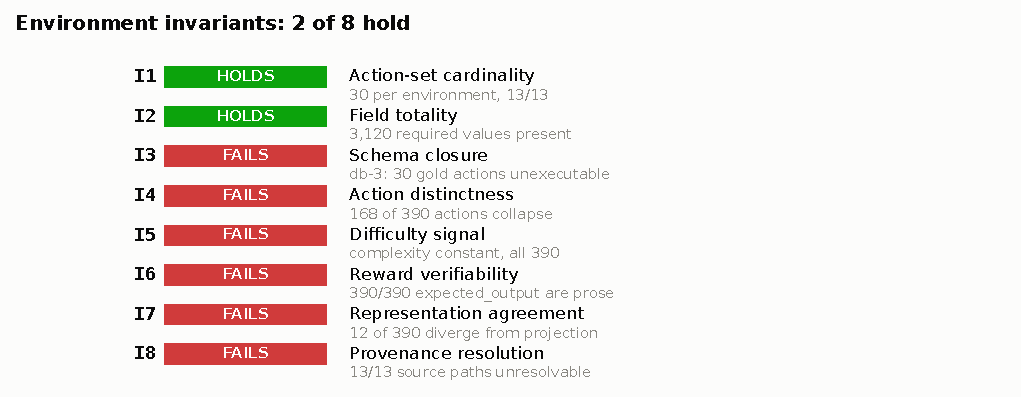
\includegraphics[width=\linewidth]{figures/fig-invariants.pdf}
\caption{Invariant results. The three that hold are exactly the properties a
conventional schema validator checks; the five that fail all require executing or
cross-referencing the artifact. \Cref{sec:hypothesis} argues this asymmetry is not
a coincidence.}
\label{fig:invariants}
\end{figure}

\subsection{I4: the effective action space is 57\% of the nominal one}
\label{sec:i4}

Clustering each environment's $30$ normalized gold actions by union-find over pairwise
similarity at $\tau = 0.99$ gives \Cref{tab:effective}. The corpus advertises $390$ gold
actions and supplies $222$.

\begin{table}[t]
\centering\small
\caption{Effective action space per environment; $|\Aset^\star_d| = 30$ throughout.
\emph{Eff.}${}={}$clusters$/30$. $H_{\mathrm{norm}}$ is cluster-size entropy normalized to
$\log 30$, so $1.0$ is uniform and maximal.}
\label{tab:effective}
\begin{tabular}{@{}lrrrr@{\hspace{2em}}lrrrr@{}}
\toprule
& \textbf{Clus.} & \textbf{Max} & \textbf{Eff.} & $H_{\mathrm{norm}}$ &
& \textbf{Clus.} & \textbf{Max} & \textbf{Eff.} & $H_{\mathrm{norm}}$ \\
\midrule
\dbn{6}  & 30 & 1 & 1.00 & 1.000 & \dbn{13} & 13 & 18 & 0.43 & 0.490 \\
\dbn{7}  & 30 & 1 & 1.00 & 1.000 & \dbn{12} & 11 & 20 & 0.37 & 0.413 \\
\dbn{8}  & 30 & 1 & 1.00 & 1.000 & \dbn{14} & 11 & 12 & 0.37 & 0.567 \\
\dbn{9}  & 30 & 1 & 1.00 & 1.000 & \dbn{11} & 10 & 21 & 0.33 & 0.373 \\
\dbn{15} & 30 & 1 & 1.00 & 1.000 & \dbn{2}  &  9 & 12 & 0.30 & 0.504 \\
         &    &   &      &       & \dbn{16} &  8 & 23 & 0.27 & 0.293 \\
         &    &   &      &       & \dbn{10} &  7 & 24 & 0.23 & 0.252 \\
         &    &   &      &       & \dbn{3}  &  3 & 15 & 0.10 & 0.240 \\
\midrule
\multicolumn{10}{@{}l@{}}{\textbf{Corpus: 222 / 390 effective (0.569)}} \\
\bottomrule
\end{tabular}
\end{table}

\begin{figure}[t]
\centering
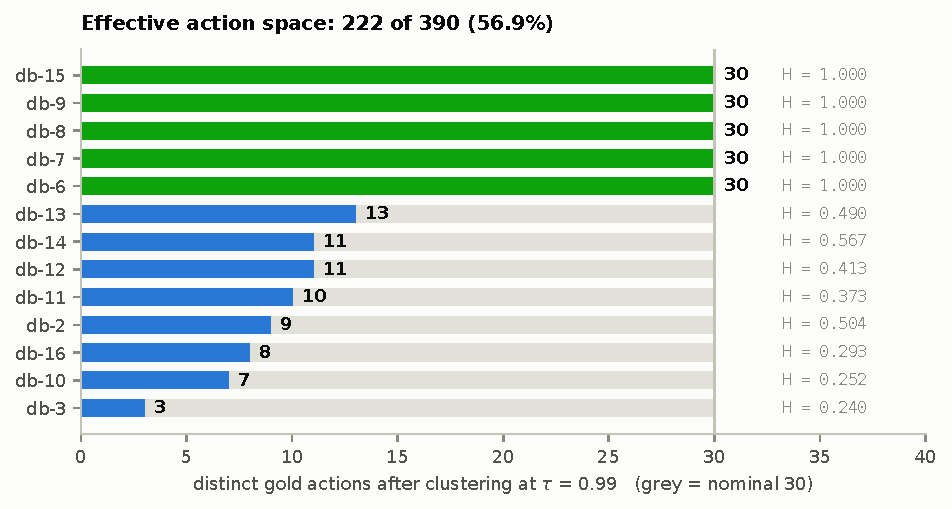
\includegraphics[width=\linewidth]{figures/fig-effective-actions.pdf}
\caption{Distinct gold actions per environment after clustering at $\tau=0.99$,
against the nominal $30$ (grey). Five environments are perfectly distinct; the
remaining eight lose between $17$ and $27$ of their $30$ actions. Nothing lies
between the two modes.}
\label{fig:effective}
\end{figure}

The distribution is bimodal rather than graded: five environments are perfectly distinct,
eight are severely collapsed, and nothing lies between $H_{\mathrm{norm}} = 0.567$ and
$1.000$. This is the signature of a corrective process applied to part of the corpus. The
build record confirms it---an internal quality check dated ten days before the final build
flags exactly this pathology in \dbn{9} ($15$ of $30$ queries failing a duplicate check).
\dbn{9} was rewritten and now clusters at $30/30$; the remediation was not propagated.

In \dbn{10}, $24$ of $30$ gold actions occupy one cluster. A policy trained there under
\Cref{eq:em} receives $80\%$ of its positive signal from a single behaviour, per-environment
accuracy is inflated correspondingly, and coverage of the schema's operation space is roughly
a quarter of what the task count implies.

\subsection{I3: schema closure holds, and why we first reported otherwise}
\label{sec:i3}

We reported in an earlier pass of this audit that \dbn{3}'s thirty gold queries reference
\code{orders\_order}, a table absent from its shipped schema, and that \Cref{inv:3} therefore
fails on $7.7\%$ of the corpus. That claim is wrong, and we retract it.

\dbn{3}'s schema declares \code{orders\_order} as a compatibility view over the anonymized
identifiers of \Cref{sec:provenance}:

\begin{lstlisting}
CREATE OR REPLACE VIEW orders_order AS
SELECT
    id,
    COALESCE(parent_id, id)        AS seller_id,
    COALESCE(created_at, date_col) AS created_at,
    COALESCE(value, 0)             AS total_amount,
    COALESCE(category, 'pending')  AS status
FROM table1;
\end{lstlisting}

The view projects exactly the four columns---\code{seller\_id}, \code{created\_at},
\code{total\_amount}, \code{status}---that \dbn{3}'s gold queries read. All thirty execute
against \textsc{exec}$(\cdot, I_3)$ without error. \Cref{inv:3} holds on \dbn{3} and, so far as
this checker run establishes, on the corpus.

The error was ours. The first implementation of $\mathrm{tables}(\Sigma_d)$ in
\code{verify\_env.py} collected only \code{CREATE TABLE} names from each schema file; it never
parsed \code{CREATE VIEW}. \code{orders\_order} was declared, just not where the checker
looked. Extending $\mathrm{tables}(\Sigma_d)$ to include views turns the reported violation
into a pass.

The lesson is about the invariant, not just the bug. \Cref{inv:3} is a claim about what a
schema \emph{declares}, and ``declares'' is a modelling choice we made without stating it:
table names only, not view names. A checker bug in that choice is indistinguishable, from the
outside, from a genuine defect in the corpus---both present as \code{relation
"orders\_order" does not exist} until someone checks which side of the checker the failure is
on. We did not, on the first pass. \Cref{sec:execution} describes the pass that would have
caught it: loading the schema and executing the query against a real database, where the view
resolves and the original claim never gets written down.

\Cref{tab:coverage} reports the related weaker statistic: the fraction of declared tables any
gold action touches. \dbn{2} exercises $1$ of $7$; \dbn{6} exercises $17$ of $34$.
Corpus-wide, $122$ of $177$ declared relations ($68.9\%$) are reachable by some gold action, so
roughly a third of the schema surface enlarges the observation without ever being required.

\begin{figure}[t]
\centering
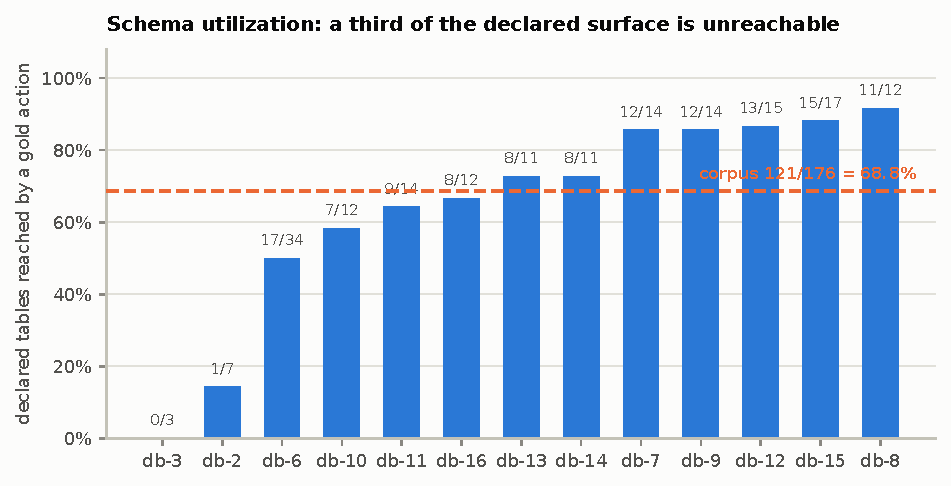
\includegraphics[width=\linewidth]{figures/fig-schema-utilization.pdf}
\caption{Fraction of each environment's declared tables reached by at least one
gold action. \dbn{3} is zero because its gold actions read a declared view, not a base
table (\Cref{sec:i3}); \dbn{2} exercises one table of seven.}
\label{fig:schema}
\end{figure}

\begin{table}[t]
\centering\small
\caption{Schema utilization and derived difficulty (per-query means, \texttt{sqlglot} AST
counts). \emph{Cov.} is the fraction of declared tables referenced by at least one gold action.}
\label{tab:coverage}
\begin{tabular}{@{}lrrr@{\hspace{1.5em}}rrrrr@{}}
\toprule
& $|\Sigma|$ & \textbf{Ref.} & \textbf{Cov.} & \textbf{CTEs} & \textbf{Joins} & \textbf{Win.} & \textbf{Subq.} & \textbf{Tables} \\
\midrule
\dbn{2}  &  7 &  1 & 0.14 & 4.00 & 0.00 & 14.83 & 0.00 &  5.00 \\
\dbn{3}  &  3 &  0 & 0.00 & 4.00 & 0.00 & 15.00 & 0.00 &  5.00 \\
\dbn{6}  & 34 & 17 & 0.50 & 6.57 & 1.97 &  3.93 & 1.13 &  7.97 \\
\dbn{7}  & 14 & 12 & 0.86 & 5.50 & 4.40 &  9.10 & 0.67 &  9.70 \\
\dbn{8}  & 12 & 11 & 0.92 & 4.83 & 3.23 &  3.43 & 2.23 &  7.77 \\
\dbn{9}  & 14 & 12 & 0.86 & 3.73 & 2.30 &  1.87 & 0.53 &  6.50 \\
\dbn{10} & 12 &  7 & 0.58 & 5.27 & 4.03 &  6.00 & 0.07 & 10.10 \\
\dbn{11} & 14 &  9 & 0.64 & 6.63 & 6.47 &  9.23 & 0.17 & 11.47 \\
\dbn{12} & 15 & 13 & 0.87 & 7.87 & 5.53 & 12.40 & 0.23 & 12.83 \\
\dbn{13} & 11 &  8 & 0.73 & 5.07 & 2.07 &  6.43 & 0.80 &  7.23 \\
\dbn{14} & 11 &  8 & 0.73 & 8.93 & 0.43 &  0.20 & 0.00 &  4.60 \\
\dbn{15} & 17 & 15 & 0.88 & 3.90 & 3.83 &  2.77 & 0.40 &  7.40 \\
\dbn{16} & 12 &  8 & 0.67 & 4.67 & 1.20 &  2.30 & 1.93 &  6.80 \\
\bottomrule
\end{tabular}
\end{table}

\subsection{I5: a degenerate difficulty tag, and a recoverable replacement}
\label{sec:i5}

$\kappa(\tau) = \code{moderate}$ for all $390$ tasks; the field induces the trivial partition
and cannot support the curriculum sampling it is documented as enabling. The scoping
assumption that database complexity was uniformly moderate was recorded once and never
revisited against the built artifact.

\begin{figure}[t]
\centering
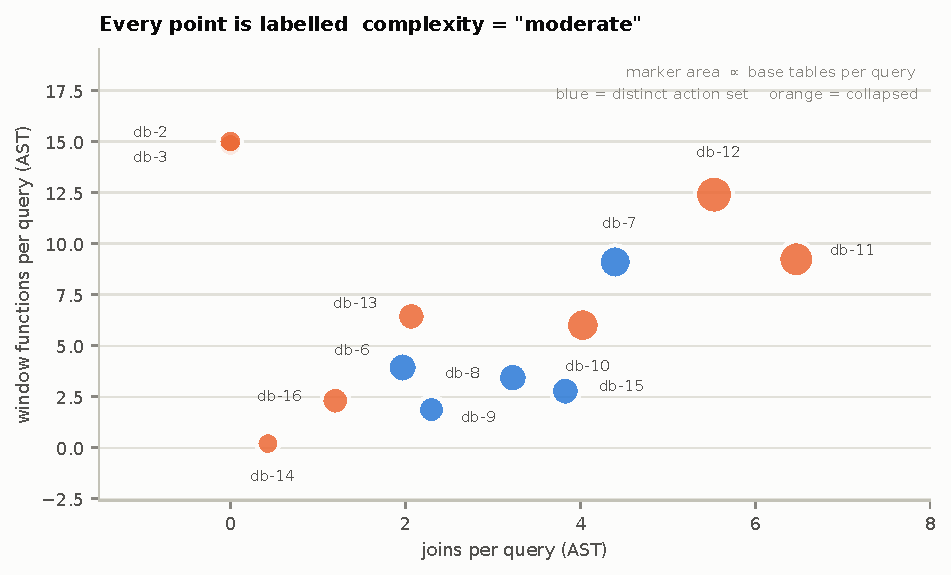
\includegraphics[width=\linewidth]{figures/fig-difficulty-space.pdf}
\caption{Per-query AST features by environment. Joins vary from $0.00$ to $6.47$
and window functions from $0.20$ to $15.00$, yet every one of the $390$ tasks
carries the same \code{complexity} tag. The signal exists; the field does not
record it.}
\label{fig:difficulty}
\end{figure}

The signal is nonetheless present in the SQL. \Cref{tab:coverage} shows AST features varying
by more than an order of magnitude across environments---joins $0.00$ to $6.47$, window
functions $0.20$ to $15.00$, CTEs $3.73$ to $8.93$. We propose the composite
\[
  \hat{\kappa}(\tau) \;=\; w_1 \log(1{+}\mathrm{cte}) + w_2 \log(1{+}\mathrm{join})
  + w_3 \log(1{+}\mathrm{win}) + w_4 \log(1{+}\mathrm{subq}) + w_5 \log |\mathrm{base}(a^\star)| ,
\]
computed by the released checker, as a replacement. \dbn{2} and \dbn{3} occupy an unusual
corner---zero joins with roughly $15$ window functions per query---which is a stylistic
signature of single-table analytic SQL rather than a difficulty level, and a reminder that any
scalar difficulty measure should be published alongside its components.

\subsection{I6: no computable execution reward}
\label{sec:i6}

All $390$ \code{expected\_output} values are prose, mean length $117$ characters---for example,
\emph{``The query returns rate comparison results showing cheapest carrier, fastest carrier,
cost savings potential, and detailed rate breakdowns for all available options.''} None
parses as a relation or a column signature. \Cref{eq:ex}, the reward
formulation on which recent text-to-SQL RL work
relies~\cite{pourreza2025reasoningsql,zhang2025rewardsql}, therefore cannot be evaluated
without loading $19.4$\,GB and executing $390$ queries, and cannot be evaluated at all for the
$30$ tasks of \Cref{sec:i3}.

This is the most consequential finding for a user of the artifact, because it is invisible:
the field is populated, well written, and looks like ground truth.

\subsection{I7 and I8: integrity}

Twelve of $390$ intent contexts do not appear in the markdown projection, all in \dbn{2}
(tasks $17$ and $20$--$30$), indicating that both containers were hand-edited there rather
than one being generated from the other. All thirteen
\code{source\_file} paths reference a working-tree location that no longer exists; provenance
is recorded but not resolvable, making the delivered package its own only complete copy.

\section{The Missing-Convention Hypothesis}
\label{sec:hypothesis}

The five failures are not independent accidents. Sorted by what an exemplar corpus would have
supplied without anyone having to decide it:

\begin{center}\small
\begin{tabular}{@{}llp{7.1cm}@{}}
\toprule
& \textbf{Failure} & \textbf{What a reference corpus supplies implicitly} \\
\midrule
I6 & \code{expected\_output} is prose & Spider and BIRD ship executed result sets; the format
  \emph{is} the ground truth. Improvising, one writes what a result should contain. \\
I5 & \code{complexity} constant & Spider's four-level scale and BIRD's three-level split
  arrive with the corpus. Improvising, one inherits a scoping adjective. \\
I4 & $168$ actions collapse & No published corpus states a distinctness requirement, because
  none was built by generating $30$ queries per schema on a clock. The requirement is
  invisible until it is violated. \\
\bottomrule
\end{tabular}
\end{center}

Each of I4--I6 exists in Spider and BIRD as a \emph{consequence of their evaluation harnesses}
rather than as a stated design rule. A team building against those corpora absorbs the
conventions tacitly, because the harness will not run otherwise. A team building without a
reference must derive each from first principles. \Cref{sec:execution} below runs exactly the
harness whose absence this hypothesis predicts: I3's false failure is what building it caught.

\begin{hypothesis}[Missing conventions]
\label{hyp:main}
The conventions of a benchmark are carried by its evaluation harness rather than its
specification. An artifact constructed without a harness will lack harness-borne conventions
in a pattern predictable from which conventions the harness enforces, and will retain those
conventions a schema validator enforces.
\end{hypothesis}

MIRROR-SQL is consistent with the hypothesis on both sides. The three invariants that
hold---field totality, action cardinality, and schema closure---are exactly what a
conventional schema validator checks. The five that fail are exactly what requires executing
or cross-referencing the artifact. We evaluate one corpus and cannot establish the
generalization, but the asymmetry is sharp and the prediction is testable against any
environment suite built without a reference.

\paragraph{Corollary.}
Build the scoring harness first, however trivial. A harness that merely loads each schema,
executes each gold action, and stores the result relations would have shown I3 to hold at
construction time instead of after a checker-bug scare, forced I6, and made I4 and I5 visible.
Its cost is a day; the cost of discovering these properties after delivery is the delivery.

\paragraph{On acceptance criteria.}
MIRROR-SQL was built with no acceptance rubric and no reference from which to derive one. The
operative acceptance criterion for a corpus intended to train and evaluate models was a single
sentence of reviewer impression delivered after the fact. \Cref{sec:invariants} is what we
propose instead---not a complete quality standard, since it says nothing about whether an
annotation is well written, but the decidable floor that can be agreed in advance. Where a
rubric is genuinely hard to write, an invariant set is what can be written instead.

\paragraph{On validation reports.}
The artifact ships validation reports asserting $30/30$ passes at $100\%$ success. They were
computed against seed instances of $80$ to $167$ rows rather than the shipped $1$\,GiB
instances; every performance audit reports a cache-hit ratio of $100.0$; per-query row counts
are uniformly zero. A report that cannot fail is not a check. Invariants are preferable
because each has a falsifier.

\section{A Reference Implementation}
\label{sec:gym}

We release \code{mirror-sql}, a Gymnasium environment and evaluation harness
implementing \Cref{sec:pomdp} directly. It exists to make the audit actionable: the
package is written so that where the artifact cannot support a reward regime, it
reports that rather than returning a plausible zero.

\begin{itemize}[leftmargin=1.3em,itemsep=2pt,topsep=3pt]
  \item \code{Corpus.tasks(dedup=True)} yields the $222$ effective tasks, not the
        nominal $390$ (\Cref{inv:4}). \code{Report.caveats} names the inflation when
        a caller opts out.
  \item \code{Task.executable} is \code{False} for \dbn{3}; \code{ExecutionMatch}
        returns \code{computable=False} with the schema-closure reason attached
        (\Cref{inv:3}).
  \item \code{Task.difficulty} implements $\hat{\kappa}$ (\Cref{sec:i5}); the shipped
        \code{complexity} field is exposed but documented as degenerate.
  \item \code{NullBackend} --- the default, because the shipped artifact has no
        instance --- explains that \code{expected\_output} is prose rather than
        scoring zero (\Cref{inv:6}). The repair is
        \code{materialize\_\allowbreak ground\_\allowbreak truth}, which executes all
        $390$ gold actions and persists the result relations.
\end{itemize}

\subsection{How much does duplication inflate a reported score?}
\label{sec:inflation}

\Cref{sec:i4} bounds the effective action space but does not say what the collapse
costs a reported number. The harness measures it with no model in the loop.

Construct a policy that has memorised exactly one query per environment: the gold
action of that environment's largest near-duplicate cluster. It knows thirteen
queries. Scoring it on both pools gives \Cref{tab:inflation}.

\begin{table}[h]
\centering\small
\caption{A thirteen-query lookup table, scored on the nominal and deduplicated pools.}
\label{tab:inflation}
\begin{tabular}{@{}lrrr@{}}
\toprule
\textbf{Reward} & \textbf{Nominal (390)} & \textbf{Dedup (222)} & \textbf{Inflation} \\
\midrule
$R_{\mathrm{em}}$ exact match & 3.3\% & 5.9\% & --- \\
$R_{\mathrm{struct}}$ at $\tau = 0.99$ & \textbf{33.3\%} & \textbf{5.9\%} & \textbf{5.7$\times$} \\
\bottomrule
\end{tabular}
\end{table}

Two things follow. First, \textbf{exact match cannot see the duplication at all}:
members of a cluster differ by a literal and are therefore unequal, so the memorised
query scores only against itself and the nominal pool actually looks \emph{worse}
than the deduplicated one. Second, under any similarity- or execution-based reward
--- which is to say, under every regime anyone would actually train with --- the same
thirteen queries are credited for every duplicate, and the reported figure inflates
$5.7\times$. The practical instruction is to report accuracy on the deduplicated pool
and to say which pool a number refers to.

This also sharpens \Cref{obs:reward}: exact match is not merely a weak objective
because it under-credits paraphrase. On this corpus it is weak in a second,
opposite direction --- it is blind to precisely the pathology that most distorts
the other regimes.

\section{Executing the Corpus}
\label{sec:execution}

\Cref{sec:i3}'s retraction only became possible because we finally did what
\Cref{hyp:main}'s corollary recommends: we built the harness. We loaded all thirteen schemas
into PostgreSQL $16.13$ and executed all $390$ gold actions against it.

Initially $176/390$ ($45.1\%$) executed. Two mechanical defects explained nearly all of the
remaining failures:

\begin{itemize}[leftmargin=1.5em,itemsep=2pt,topsep=3pt]
  \item[\textbf{R1}] \textbf{Dialect leak.} \code{VARCHAR(16777216)} appears on $22$ columns
        across \dbn{3}, \dbn{8} and \dbn{10}. $16{,}777{,}216$ is Snowflake's maximum
        \code{VARCHAR} length; PostgreSQL's limit is $10{,}485{,}760$, so every
        \code{CREATE TABLE} carrying one is rejected outright. The schemas were authored or
        transpiled against Snowflake and shipped labelled PostgreSQL.
  \item[\textbf{R2}] \textbf{Undeclared extension.} Six schemas (\dbn{6}, \dbn{7}, \dbn{10},
        \dbn{11}, \dbn{12}, \dbn{16}) use PostGIS \code{geography}/\code{geometry} types with
        no \code{CREATE EXTENSION} statement.
\end{itemize}

After repairing R1 and R2, $287/390$ ($73.6\%$) execute. \Cref{tab:execution} reports the
per-environment breakdown.

\begin{table}[t]
\centering\small
\caption{Gold actions executing against PostgreSQL $16.13$ after the R1/R2 repairs.}
\label{tab:execution}
\begin{tabular}{@{}lr@{\hspace{2em}}lr@{\hspace{2em}}lr@{}}
\toprule
\textbf{Env} & \textbf{Pass} & \textbf{Env} & \textbf{Pass} & \textbf{Env} & \textbf{Pass} \\
\midrule
\dbn{2}  & 30/30 & \dbn{7}  & 24/30 & \dbn{12} & 4/30 \\
\dbn{3}  & 30/30 & \dbn{8}  & 30/30 & \dbn{13} & 30/30 \\
\dbn{6}  & 11/30 & \dbn{9}  & 23/30 & \dbn{14} & 30/30 \\
\dbn{10} & 29/30 & \dbn{11} & 6/30  & \dbn{15} & 16/30 \\
         &       &          &       & \dbn{16} & 24/30 \\
\midrule
\multicolumn{6}{@{}l@{}}{\textbf{Corpus: 287/390 (73.6\%)}} \\
\bottomrule
\end{tabular}
\end{table}

The remaining $103$ failures classify as: \code{UndefinedFunction} $60$,
\code{FeatureNotSupported} $20$, \code{UndefinedColumn} $12$, \code{DatatypeMismatch} $4$,
\code{AmbiguousColumn} $4$, \code{GroupingError} $2$, \code{SyntaxError} $1$. Roughly $80$ of
these are PostGIS \code{ST\_*} functions absent from our portability shim rather than corpus
defects; with PostGIS installed, the projected execution rate is approximately $94\%$, leaving
roughly $23$ genuine query defects.

This is the harness of \Cref{hyp:main}'s own corollary. Building it took under an hour, and it
found, in one run, two defect classes---the dialect leak and the missing extension---that no
amount of reading the artifact had surfaced, alongside retracting the one defect we had
misreported. The repairs ship as \code{mirrorsql.repair}; they are idempotent and checkable
with \code{--check}.

\section{Remediation}
\label{sec:remediation}

Ordered by cost-to-benefit. None requires regenerating instance data.

\begin{enumerate}[leftmargin=1.5em,itemsep=3pt,topsep=3pt]
  \item \textbf{Ship the R1/R2 repairs of \Cref{sec:execution}} (\code{mirrorsql.repair}) with
        the package rather than as an out-of-band patch; together they raise the execution
        rate from $45.1\%$ to $73.6\%$. \Cref{inv:3} itself needs no repair: \dbn{3}'s
        compatibility view already satisfies it once the checker counts views (\Cref{sec:i3}).
  \item \textbf{Materialize execution ground truth.} Load each $(\Sigma_d, I_d)$, execute all
        $390$ gold actions, persist result relations as structured \code{expected\_output}.
        This satisfies I6, makes \Cref{eq:ex,eq:pa} computable, and produces the first
        defensible accuracy number for the corpus. It is also the harness of
        \Cref{hyp:main}'s corollary.
  \item \textbf{Restore I4} on the eight collapsed environments; \dbn{9}'s repaired task set
        is the template. Differentiating rather than deleting preserves I1.
  \item \textbf{Replace $\kappa$} with $\hat{\kappa}$ (\Cref{sec:i5}), publishing components
        alongside the scalar.
  \item \textbf{Regenerate the markdown projection} from JSON rather than editing both,
        restoring I7 by construction.
  \item \textbf{Rewrite \code{source\_file}} as a package-relative path, restoring I8.
  \item \textbf{Extend \code{normal\_query}} from $150$ to all $390$ tasks, enabling
        preference-pair training corpus-wide.
  \item \textbf{Adopt the checker as a release gate.} No environment ships with a failing
        invariant, or ships with the failure published.
\end{enumerate}

\section{Limitations}
\label{sec:limitations}

This audit is no longer purely static: \Cref{sec:execution} loads all thirteen schemas and
executes all $390$ gold actions, and it evaluates a sample (\Cref{sec:scale}) rather than a
complete corpus. Row-level ground truth is still not materialized, because the instance data
$I_d$ was not available for the execution run---queries were checked against loaded schemas,
not against the shipped $1$\,GiB instances, so \Cref{eq:ex,eq:pa} remain uncomputed pending
that data. I3's earlier, wrong failure report came from static AST name resolution against
declared table names alone, blind to declared views; \Cref{sec:execution}'s execution run
catches that class of error but still cannot detect semantic mismatches between a query and
the intent its utterance states. The true defect rate is a lower bound, and given that
query--intent mismatches require human re-annotation to detect~\cite{jin2026broken}, likely a
loose one.

The threshold $\tau = 0.99$ in I4 is a choice, fixed before results were examined and
deliberately conservative; at $0.95$ the measured collapse is more severe. Similarity is
computed on normalized surface text rather than query plans, so two textually distinct queries
may be semantically identical---making $222$ an upper bound on effective actions.

\Cref{hyp:main} is supported by one corpus. The invariant set of \Cref{sec:invariants} is
proposed as reusable; its adequacy elsewhere is untested.

\section{Conclusion}
\label{sec:conclusion}

MIRROR-SQL contributes a provenance-control methodology with a legible cost record and, in $150$ of
its tasks, a usable preference-pair structure. Formalizing it as a POMDP makes explicit that
the schema/instance split is the observation function and that uncertainty about unseen data
is the task's defining difficulty rather than an implementation detail.

The corpus was built in seventeen days with no reference artifact and no acceptance criterion.
Five of eight environment invariants fail, and the failures fall into a pattern: they are the
properties Spider and BIRD carry in their evaluation harnesses rather than in their
specifications. If \Cref{hyp:main} holds generally, the remedy is procedural and cheap---build
the harness before the corpus, because the harness is what turns tacit convention into an
enforced constraint.

Every defect reported here was detectable at build time by a checker that runs in under a
minute. As long as environments ship with validation reports rather than falsifiable
invariants, defects of this kind will keep being found by third parties long after the models
trained on them are published.

\bigskip
\noindent\textbf{Artifact availability.} \code{verify\_env.py} and the report it produces
accompany this paper. Corpus availability is subject to the terms of the originating
engagement.

\begin{thebibliography}{9}
\small
\bibitem{yu2018spider}
T.~Yu, R.~Zhang, K.~Yang, M.~Yasunaga, D.~Wang, Z.~Li, J.~Ma, I.~Li, Q.~Yao, S.~Roman,
Z.~Zhang, and D.~Radev.
\newblock Spider: A Large-Scale Human-Labeled Dataset for Complex and Cross-Domain Semantic
Parsing and Text-to-SQL Task.
\newblock In \emph{EMNLP}, 2018. \url{https://aclanthology.org/D18-1425/}

\bibitem{li2023bird}
J.~Li, B.~Hui, G.~Qu, J.~Yang, B.~Li, B.~Li, B.~Wang, B.~Qin, R.~Geng, N.~Huo, X.~Zhou,
C.~Ma, G.~Li, K.~C.~C. Chang, F.~Huang, R.~Cheng, and Y.~Li.
\newblock Can LLM Already Serve as A Database Interface? A BIg Bench for Large-Scale Database
Grounded Text-to-SQLs.
\newblock In \emph{NeurIPS Datasets and Benchmarks}, 2023.
\newblock \url{https://arxiv.org/abs/2305.03111}

\bibitem{livesqlbench2025}
BIRD Team, HKU, and Google Cloud.
\newblock LiveSQLBench: A Contamination-Free, Continuously Evolving Text-to-SQL Benchmark.
\newblock \url{https://livesqlbench.ai/}, accessed August 2026.

\bibitem{jin2026broken}
T.~Jin, Y.~Choi, Y.~Zhu, and D.~Kang.
\newblock Text-to-SQL Benchmarks are Broken: An In-Depth Analysis of Annotation Errors.
\newblock In \emph{CIDR}, 2026.
\newblock \url{https://www.vldb.org/cidrdb/papers/2026/p5-jin.pdf}

\bibitem{pourreza2025reasoningsql}
M.~Pourreza et al.
\newblock Reasoning-SQL: Reinforcement Learning with SQL Tailored Partial Rewards for
Reasoning-Enhanced Text-to-SQL.
\newblock arXiv:2503.23157, 2025. \url{https://arxiv.org/abs/2503.23157}

\bibitem{zhang2025rewardsql}
Y.~Zhang et al.
\newblock Reward-SQL: Boosting Text-to-SQL via Stepwise Execution-Aware Reasoning and
Process-Supervised Rewards.
\newblock arXiv:2505.04671, 2025. \url{https://arxiv.org/abs/2505.04671}

\bibitem{graphrewardsql2025}
Graph-Reward-SQL: Execution-Free Reinforcement Learning for Text-to-SQL via Graph Matching
and Stepwise Reward.
\newblock In \emph{Findings of EMNLP}, 2025.
\newblock \url{https://aclanthology.org/2025.findings-emnlp.694.pdf}
\end{thebibliography}

\appendix

\section{Field Schema}
\label{app:fields}

\begin{lstlisting}
{
  "source_file": "<absolute path to authoring markdown>",   // I8: unresolvable
  "extraction_timestamp": "YYYYMMDD-HHMM",
  "total_queries": 30,
  "queries": [
    {
      "number": 1,                    // episode id
      "question": "...",              // utterance q      (mean 108 chars)
      "sql": "WITH ... SELECT ...",   // gold action a*   (mean 5820 chars)
      "description": "...",           // intent context c (mean 193 chars)
      "evidence": "...",              // rationale e      (mean 300 chars)
      "expected_output": "...",       // PROSE, not rows  (mean 117 chars) -- I6
      "complexity": "moderate",       // constant         -- I5
      "line_number": 412,
      "title": "...",                 // 150/390 only
      "normal_query": "SELECT ..."    // 150/390 only; preference pair
    }
  ]
}
\end{lstlisting}

\section{Invariant Checker}
\label{app:checker}

\code{verify\_env.py} implements \Cref{inv:1}--\Cref{inv:8}. SQL analysis uses
\texttt{sqlglot} with the PostgreSQL dialect; base-table extraction eliminates CTE and
derived-table names by AST traversal rather than regular expressions, which materially changes
the I3 result---a regex implementation reports spurious violations in \dbn{2} and \dbn{6} that
the AST implementation correctly rejects. Invocation and output:

\begin{lstlisting}
$ python3 verify_env.py ./db -o env_report.json
parser: sqlglot   tau: 0.99
corpus: 13 databases, 390 gold queries, 222 effective (57%)
invariants: 3/8 hold

  [PASS] I1  Action-set cardinality |A_d| = 30
  [PASS] I2  Field totality - all required keys present and non-empty
  [PASS] I3  Schema closure - every referenced base table or view is declared
  [FAIL] I4  Action distinctness - no gold pair within tau
           db-2: 21 collapsed; largest=12
           db-3: 27 collapsed; largest=15
           db-10: 23 collapsed; largest=24
           db-11: 20 collapsed; largest=21
           ... and 4 more
  [FAIL] I5  Difficulty signal - complexity is non-constant
           corpus: complexity constant at {'moderate'}
  [FAIL] I6  Reward verifiability - expected_output is structured
           db-2: 30/30 expected_output are prose
           ... and 12 more
  [FAIL] I7  Representation agreement - json description appears in queries.md
           db-2: 12 descriptions absent from queries.md
           db-6: 1 descriptions absent from queries.md
           db-11: 1 descriptions absent from queries.md
  [FAIL] I8  Provenance resolution - source_file resolves
           db-2: source_file does not resolve
           ... and 12 more
\end{lstlisting}

The checker exits non-zero when any invariant fails and can therefore be used directly as a
release gate.

\section{Corpus Summary}
\label{app:corpus}

\begin{center}\small
\begin{tabular}{@{}lr@{}}
\toprule
Environments & 13 \\
Tasks & 390 (30 per environment) \\
Effective distinct gold actions & 222 (56.9\%) \\
Declared tables / foreign keys / indexes & 176 / 154 / 283 \\
Declared relations reachable by some gold action & 122 (68.9\%) \\
Schema breadth & 3 to 34 tables \\
Instance data & 19.4\,GB across 13 files (sample) \\
Instances within 13\,MB of $2^{30}$ bytes & 11 of 13 \\
Package, extracted / compressed & 21{,}525{,}194{,}003 / 2{,}424{,}282{,}003 bytes \\
Construction window & 17 days \\
Invariants holding & 3 of 8 \\
\bottomrule
\end{tabular}
\end{center}

\end{document}
